\chapter{Gestion d'universités : UniversityBundle}

Ces fonctionnalités sont présentés dans le UniversityBundle. Ce bundle contient l'ensemble des fonction affectant les universités. La majorité des fonctions présentes sont relatives aux administrateurs puisqu'il s'agit principalement d'ajout et de modification d'université.

\section{Ajout d'université (Administrateur)}

Les administrateurs peuvent ajouter de nouvelles universités à la base de données grâce à un import CSV. Ce fichier doit être formater de la façon suivante : Nom,Pays,Département,nombredeplace,[semestre] (cf figure \ref{au}).
\smallbreak
La liste de semestre n'a besoin d'être remplie que si on veut limiter le nombres de semestres auxquels la destination est accessible.

\begin{figure}[H]
	\centering
	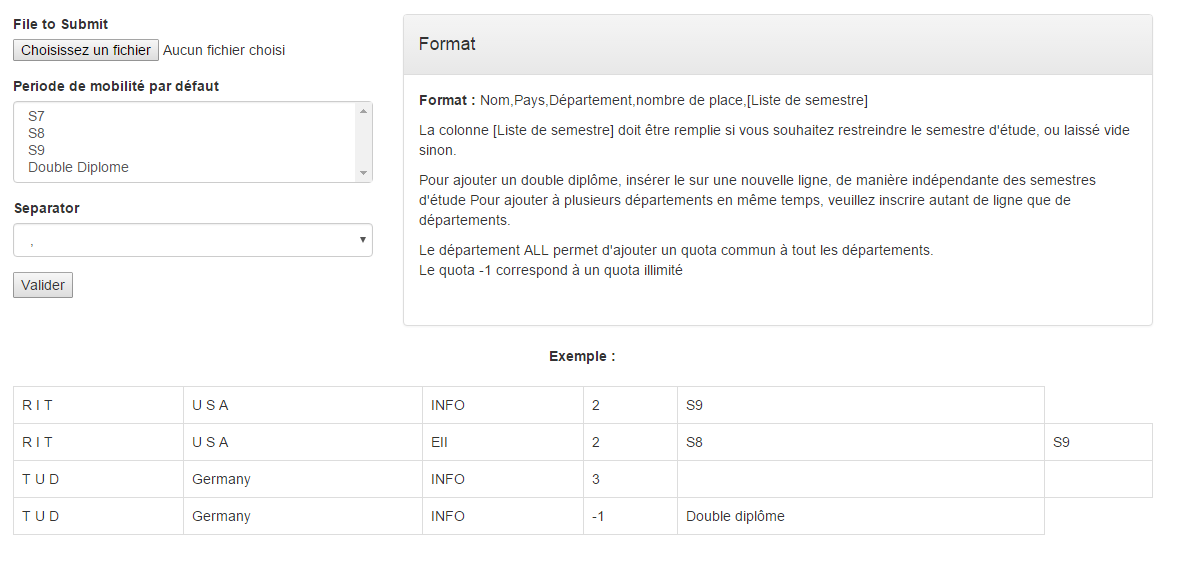
\includegraphics[scale=0.35]{images/au.png}
	\caption{Ajout de nouvelles universités}
	\label{au}
\end{figure}

\section{Modification des universités (Adminstrateur)}

Même après l'ajout d'une université, il est possible de modifier les paramètres liés à celle-ci. Il est possible de modifier les semestres disponible et le nombre de places disponibles (cf figure \ref{mu}).

\begin{figure}[H]
	\centering
	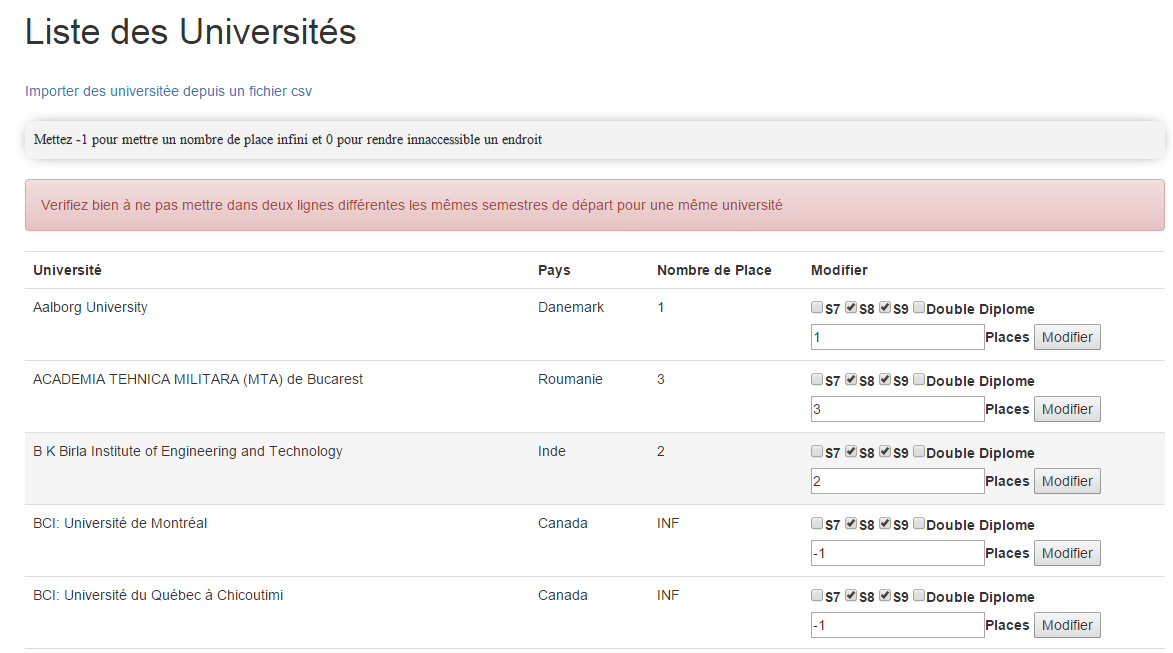
\includegraphics[scale=0.35]{images/mu.png}
	\caption{Modification des universités}
	\label{mu}
\end{figure}

\section{Résumé de l'université}

Disponible pour tout les utilisateur, un résumé de l'université. Il est possible de voir toutes les personnes qui sont parti en mobilité dans cette université mais aussi la liste des semestre disponible, le nombre de places disponibles (cf figure \ref{fru}).
\smallbreak
Par la suite, il sera possible aux élèves de mettre des commentaire sur l'université ainsi qu'au administrateur de mettre des commentaire plus particulier comme la nécessité d'avoir un diplôme particulier pour aller dans cette université.

\begin{figure}[H]
	\centering
	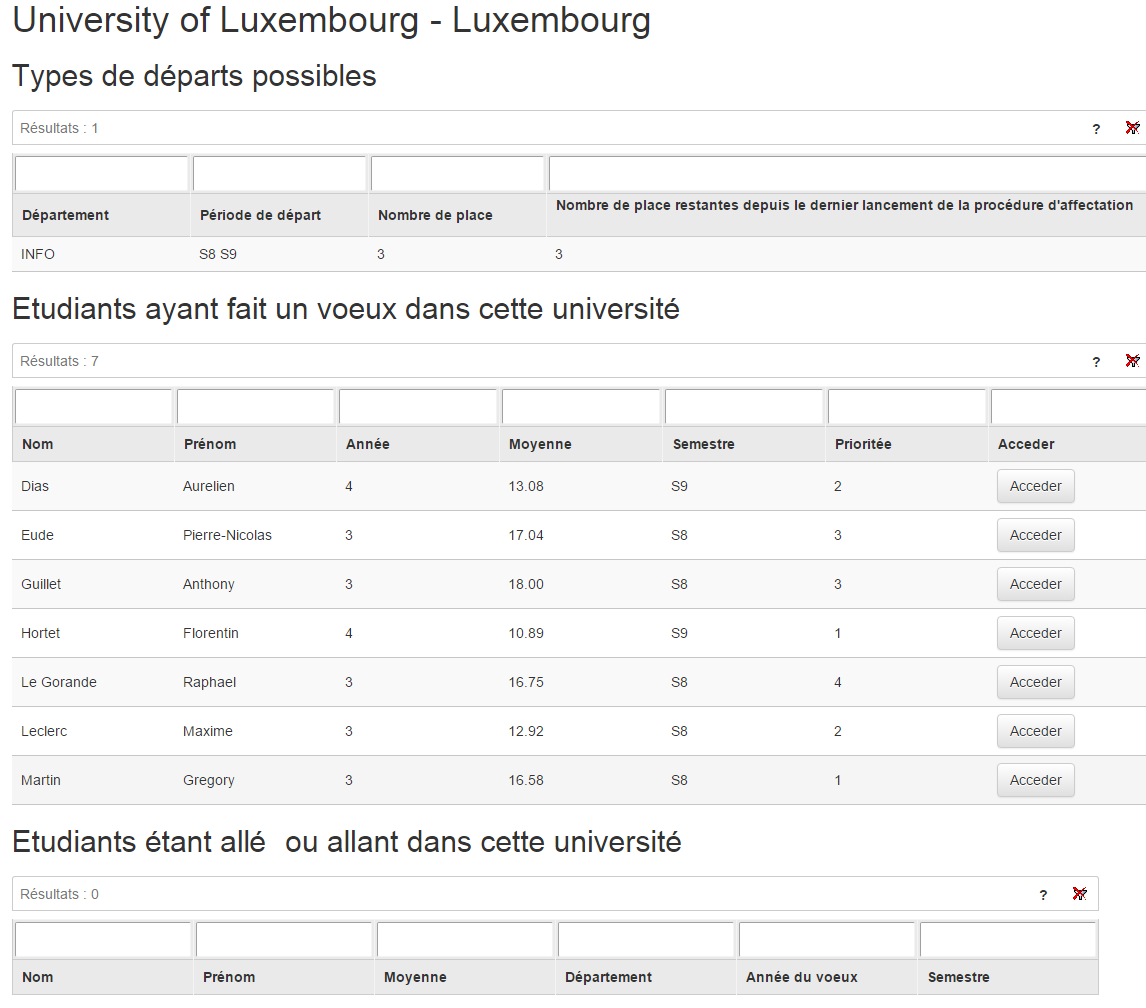
\includegraphics[scale=0.30]{images/fru.png}
	\caption{Page résumé d'une université}
	\label{fru}
\end{figure}


